\documentclass[12pt,a4paper]{article}

\usepackage[utf8]{inputenc}
\usepackage[spanish]{babel}
\usepackage{amsmath,amssymb}
\usepackage{graphicx}
\usepackage{booktabs}
\usepackage{float}
\usepackage{caption}
\usepackage{subcaption}
\usepackage[hidelinks]{hyperref}
\usepackage{geometry}
\usepackage{siunitx}
\usepackage{array}
\usepackage{parskip}
\usepackage{textcomp}

\geometry{margin=2.5cm}

\title{
  \large IOR442 Sistemas de Control\\[0.5em]
  \Large \textbf{Trabajo Práctico Nro. 1}\\[0.3em]
  \large Diseño de Controladores con Root Locus y Respuesta en Frecuencia
}
\author{
  Juan Kaplan \and Lucio Luque Materazzi \and Teo Manuel Kaucher
}
\date{Abril 2026}

\begin{document}

\maketitle
\tableofcontents
\newpage

% ====================================================================
\section{Ejercicio 1: Sistema de Control de un Rotor de Aspas}
% ====================================================================

\subsection{Parte A: Análisis del Sistema}

% -------------------------------------------------------
\subsubsection*{a) Función de transferencia y ecuaciones de estado}
% -------------------------------------------------------

La dinámica del motor de corriente continua está dada por:
\begin{align}
  L\,\frac{di(t)}{dt} + R\,i(t) + K_e\,\omega(t) &= V(t) \label{eq:elec}\\
  J\,\frac{d\omega(t)}{dt} + B\,\omega(t) &= K_t\,i(t) \label{eq:mec}\\
  \omega(t) &= \frac{d\theta(t)}{dt} \label{eq:kinem}
\end{align}

Aplicando la transformada de Laplace a las ecuaciones anteriores y despejando $\Theta(s)/V(s)$:

\[
  I(s)(Ls + R) + K_e\,s\,\Theta(s) = V(s)
\]
\[
  (Js^2 + Bs)\,\Theta(s) = K_t\,I(s) \implies I(s) = \frac{(Js^2+Bs)\,\Theta(s)}{K_t}
\]

Sustituyendo $I(s)$ en la ecuación eléctrica:
\[
  \frac{(Js^2+Bs)(Ls+R)}{K_t}\,\Theta(s) + K_e\,s\,\Theta(s) = V(s)
\]

\[
  \boxed{G(s) = \frac{\Theta(s)}{V(s)} = \frac{K_t}{s\!\left[LJ\,s^2 + (LB+RJ)\,s + K_tK_e + RB\right]}}
\]

Reemplazando con los valores numéricos $L=0.15$, $R=0.7$, $K_e=0.1$, $J=0.02$, $B=0.25$, $K_t=0.25$:
\begin{align*}
  LJ &= 0.003, &
  LB+RJ &= 0.0515, &
  K_tK_e + RB &= 0.2
\end{align*}

\[
  G(s) = \frac{0.25}{s\!\left[0.003\,s^2 + 0.0515\,s + 0.2\right]}
\]

\textbf{Ecuaciones en variables de estado.}
Definiendo $X_1 = i$, $X_2 = \omega$, $X_3 = \theta$, las ecuaciones~\eqref{eq:elec}--\eqref{eq:kinem} se escriben en forma matricial como:

\[
  \dot{\mathbf{x}} =
  \begin{bmatrix}
    -R/L & -K_e/L & 0 \\
    K_t/J & -B/J & 0 \\
    0 & 1 & 0
  \end{bmatrix}
  \mathbf{x}
  +
  \begin{bmatrix} 1/L \\ 0 \\ 0 \end{bmatrix}
  V
  =
  \begin{bmatrix}
    -4.667 & -0.667 & 0 \\
    12.5 & -12.5 & 0 \\
    0 & 1 & 0
  \end{bmatrix}
  \mathbf{x}
  +
  \begin{bmatrix} 6.667 \\ 0 \\ 0 \end{bmatrix}
  V
\]
\[
  y = \begin{bmatrix} 0 & 0 & 1 \end{bmatrix}\mathbf{x}
\]

% -------------------------------------------------------
\subsubsection*{b) Márgenes de ganancia y fase a lazo abierto}
% -------------------------------------------------------

Evaluando la planta $G(s)$ obtenida, se calculan los márgenes de estabilidad a lazo abierto:

\begin{center}
\begin{tabular}{lc}
  \toprule
  Parámetro & Valor \\
  \midrule
  Margen de ganancia (MG) & $22.76\ \si{dB}$ \\
  Margen de fase (MF)     & $72.22^\circ$ \\
  \bottomrule
\end{tabular}
\end{center}

Dado que valores adecuados requieren $\text{MG} > 6\ \si{dB}$ y $\text{MF} \approx 30^\circ$--$60^\circ$, el sistema ya posee márgenes buenos. Por lo tanto, no es estrictamente necesario introducir un compensador por motivos de estabilidad.

% -------------------------------------------------------
\subsubsection*{c) Sistema a lazo cerrado con perturbación tipo escalón (referencia escalón unitario)}
% -------------------------------------------------------

Considerando el sistema en lazo cerrado con realimentación unitaria, la salida ante una referencia $V(s)$ y una perturbación de carga $N(s)$ es:

\[
  E(s) = V(s) - \Theta(s)
\]

\[
  \Theta(s) = G(s)\bigl(E(s) + N(s)\bigr)
\]

\[
  \Theta(s) = G(s)\bigl(V(s) - \Theta(s) + N(s)\bigr)
\]

\[
  (1 + G(s))\,\Theta(s) = G(s)\,V(s) + G(s)\,N(s)
\]

\[
  \Theta(s) = \underbrace{\frac{G(s)}{1+G(s)}}_{\Theta/V}\,V(s)
             + \underbrace{\frac{G(s)}{1+G(s)}}_{\Theta/N}\,N(s)
\]

Evaluando numéricamente:
\[
  \frac{\Theta(s)}{V(s)} = \frac{\Theta(s)}{N(s)}
  = \frac{0.25}{0.003\,s^3 + 0.0515\,s^2 + 0.2\,s + 0.25}
\]

Con $V(s) = 1/s$ (escalón unitario) y $N(s) = 0.1/s$ (perturbación de magnitud $0.1$), la respuesta se muestra en la Fig.~\ref{fig:ej1_step_dist}.

\begin{figure}[H]
  \centering
  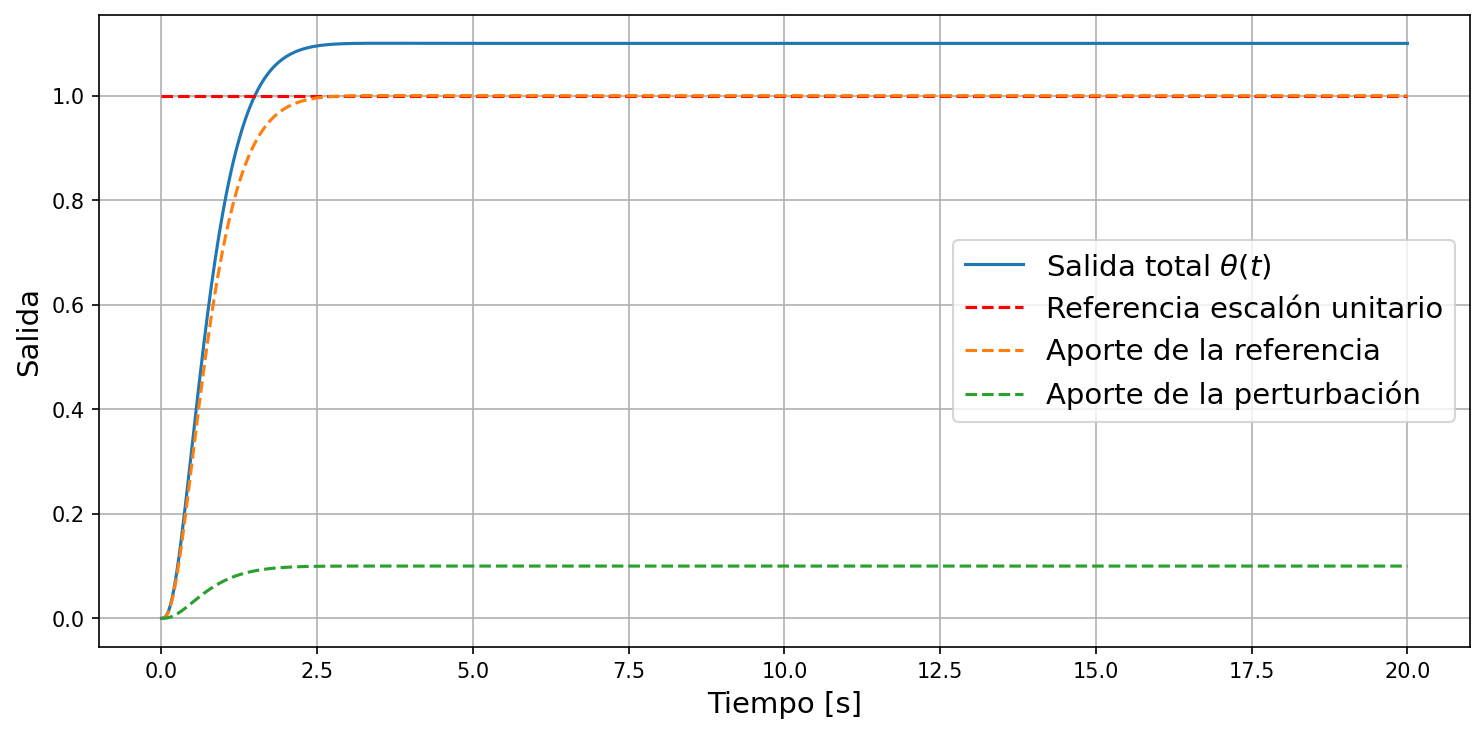
\includegraphics[width=0.85\textwidth]{figures/ej1_step_disturbance.png}
  \caption{Respuesta del sistema a lazo cerrado ante escalón unitario y perturbación constante de magnitud $0.1$.}
  \label{fig:ej1_step_dist}
\end{figure}

Se observa que el sistema sigue al escalón con error cero, pero la perturbación introduce un desplazamiento constante en la salida total por encima de la referencia. Esto ocurre porque $\lim_{s\to 0} s \cdot \frac{G(s)}{1+G(s)} \cdot \frac{0.1}{s} = 0.1$, es decir, el sistema es de Tipo 1 y no puede rechazar perturbaciones constantes en lazo cerrado sin compensación adicional.

% -------------------------------------------------------
\subsubsection*{d) Sistema a lazo cerrado con perturbación tipo escalón (referencia rampa unitaria)}
% -------------------------------------------------------

Manteniendo la misma perturbación constante de magnitud $0.1$, pero ahora con una referencia rampa unitaria $V(s) = 1/s^2$, la respuesta se presenta en la Fig.~\ref{fig:ej1_ramp_dist}.

\begin{figure}[H]
  \centering
  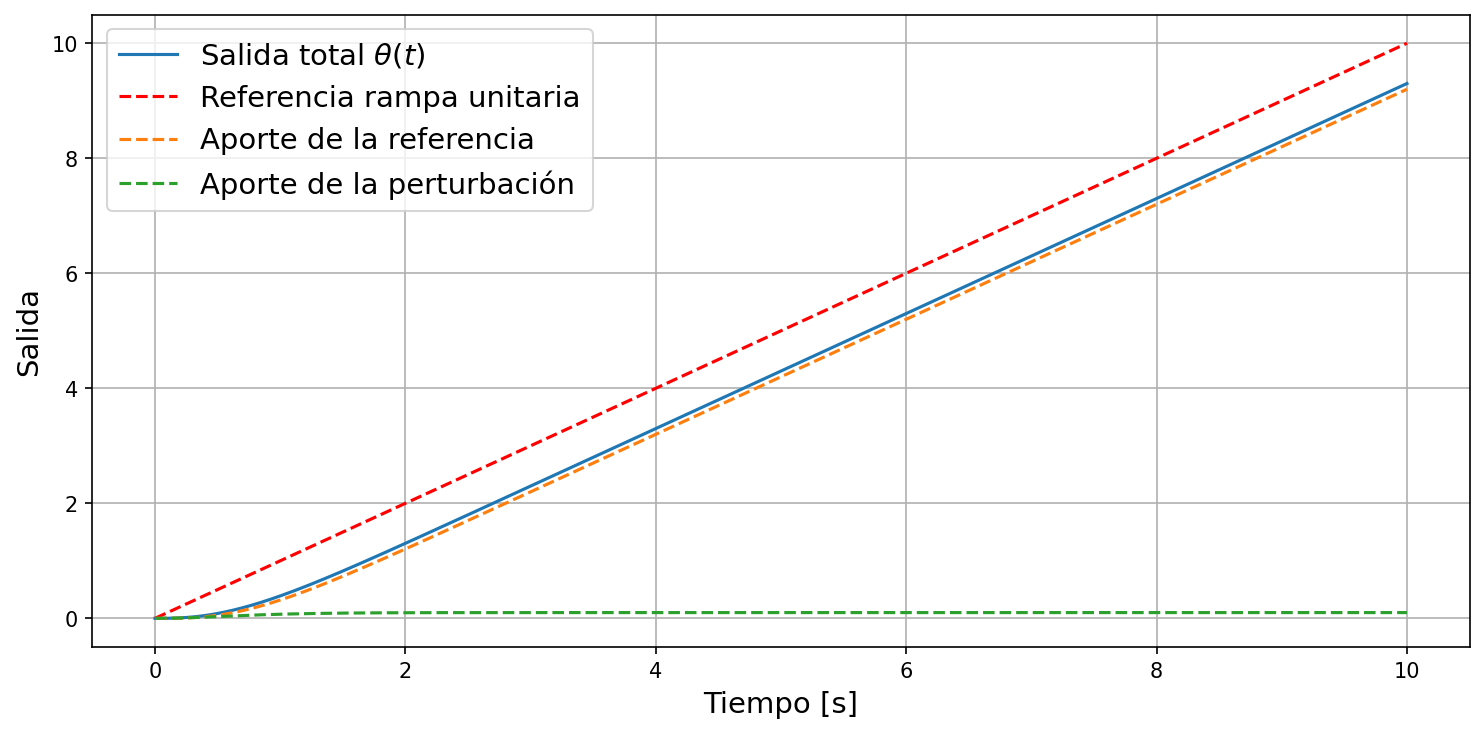
\includegraphics[width=0.85\textwidth]{figures/ej1_ramp_disturbance.png}
  \caption{Respuesta del sistema a lazo cerrado ante rampa unitaria y perturbación constante de magnitud $0.1$.}
  \label{fig:ej1_ramp_dist}
\end{figure}

En este caso el sistema presenta un error de velocidad constante, ya que el sistema es de Tipo~1 y no puede seguir una rampa con error nulo. La perturbación genera un offset adicional que reduce levemente el error de velocidad total, pero no lo elimina.

% -------------------------------------------------------
\subsubsection*{e) Propuesta de controlador para cada caso}
% -------------------------------------------------------

Al estudiar los márgenes de ganancia y fase se observó que el sistema ya posee estabilidad ante perturbaciones. Esto se ve reflejado en los gráficos de respuesta al escalón y rampa, donde el sistema tiene un error constante y no diverge ni oscila.

Tanto para el escalón como para la rampa, para minimizar el error de estado estacionario se puede usar un controlador \textbf{PI}, que agrega un término integrador capaz de mitigar el error ante el escalón y la rampa.

% ====================================================================
\subsection{Parte B: Diseño del Sistema de Control}
% ====================================================================

% -------------------------------------------------------
\subsubsection*{a) Desempeño a lazo cerrado sin compensación ($C(s)=1$)}
% -------------------------------------------------------

Considerando el sistema en lazo cerrado con $C(s)=1$, ante una entrada escalón unitario y una perturbación de magnitud $0.2$ (el $20\%$ de la referencia), se obtienen los siguientes valores:

\begin{center}
\begin{tabular}{lcc}
  \toprule
  Parámetro & Valor obtenido & Requisito \\
  \midrule
  Tiempo de establecimiento ($t_s$, 2\%) & $2.052\ \si{s}$ & $\leq 7.5\ \si{s}$ \checkmark \\
  Sobrepico máximo ($M_p$)               & $0.0\ \%$     & $\leq 15\ \%$ \checkmark \\
  Error en estado estacionario           & $20\ \%$          & $< 5\ \%$ \texttimes \\
  \bottomrule
\end{tabular}
\end{center}

La respuesta al escalón se muestra en la Fig.~\ref{fig:ej1_cl_step}.

\begin{figure}[H]
  \centering
  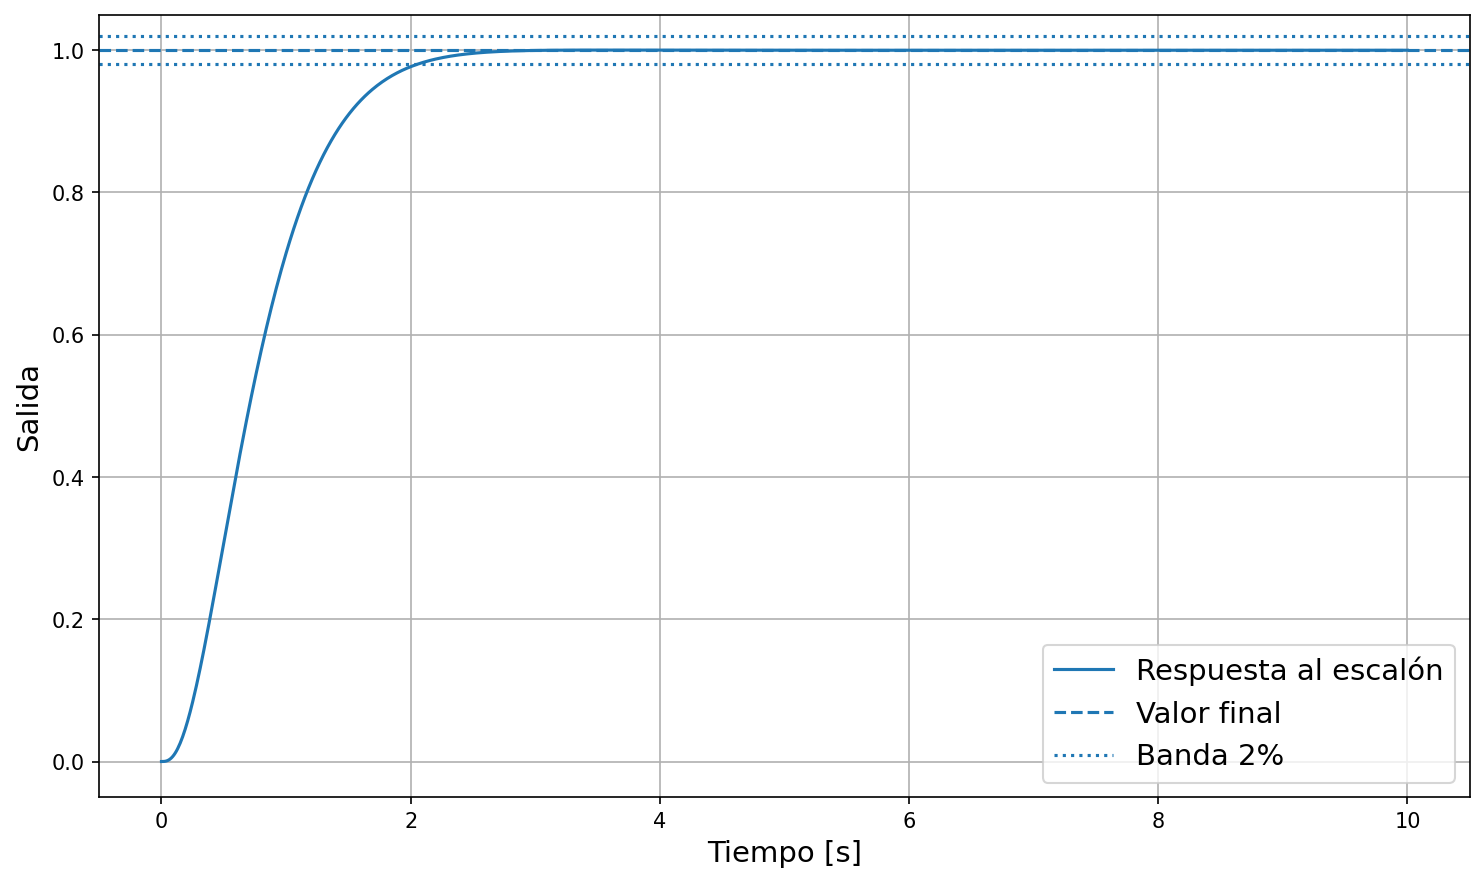
\includegraphics[width=0.80\textwidth]{figures/ej1_closed_loop_step.png}
  \caption{Respuesta al escalón unitario a lazo cerrado sin compensador, con banda del $2\%$.}
  \label{fig:ej1_cl_step}
\end{figure}

El error del $20\%$ se verifica analíticamente. Con perturbación de magnitud $0.2$:

\[
  E(s) = R(s) - \Theta(s)
\]

\[
  e_{ss} = \lim_{s\to 0} s\,E(s)
\]

\[
  e_{ss} = \lim_{s\to 0} s\!\left[\frac{1}{s} - \frac{\Theta(s)}{V(s)}\frac{1}{s} - \frac{\Theta(s)}{N(s)}\frac{0.2}{s}\right]
\]

\[
  e_{ss} = \lim_{s\to 0} s\left[\frac{1}{s}
    - \frac{0.25}{0.003s^3 + 0.0515s^2 + 0.2s + 0.25}\cdot\frac{1}{s}
    - \frac{0.25}{0.003s^3 + 0.0515s^2 + 0.2s + 0.25}\cdot\frac{0.2}{s}
  \right]
\]

\[
  e_{ss} = 1 - 1 - 0.2 = 0.2 \quad (20\%)
\]



Si bien el tiempo de establecimiento y el sobrepico cumplen con las especificaciones, el error de precisión ante perturbación constante es inaceptable. Es necesario introducir un controlador.

% -------------------------------------------------------
\subsubsection*{b) Diseño del controlador PI por root locus}
% -------------------------------------------------------

Se plantea el uso de un controlador PI de la forma:
\[
  C(s) = K_p + \frac{K_i}{s}
\]

\textbf{Transferencia a lazo cerrado con PI.}
Con realimentación unitaria y perturbación de carga $N(s)$, la salida es:

\begin{align*}
  \theta(s) &= \bigl[(V(s)-\theta(s))C(s) + N(s)\bigr]G(s) \\
  (1 + G(s)C(s))\,\theta(s) &= G(s)C(s)\,V(s) + G(s)\,N(s) \\[4pt]
  \theta(s) &= \underbrace{\frac{G(s)C(s)}{1+G(s)C(s)}}_{\Theta/V}\,V(s)
             + \underbrace{\frac{G(s)}{1+G(s)C(s)}}_{\Theta/N}\,N(s)
\end{align*}

Sustituyendo $G(s) = \dfrac{0.25}{s[0.003s^2+0.0515s+0.2]}$ y $C(s) = K_p + K_i/s$:

\begin{align}
  \frac{\Theta(s)}{V(s)} &= \frac{0.25(sK_p + K_i)}{0.003s^4 + 0.0515s^3 + 0.2s^2 + 0.25K_p s + 0.25K_i} \label{eq:TvPI}\\[4pt]
  \frac{\Theta(s)}{N(s)} &= \frac{0.25\,s}{0.003s^4 + 0.0515s^3 + 0.2s^2 + 0.25K_p s + 0.25K_i} \label{eq:TnPI}
\end{align}

\textbf{Demostración de $e_{ss}=0$.} Para una referencia escalón (\(R(s)=1/s\)) y una perturbación constante de magnitud $0.2$, definimos
\[
  E(s)=R(s)-\Theta(s)
\]
y
\[
  e_{ss}=\lim_{s\to 0} s\,E(s).
\]

Sustituyendo las expresiones de entrada y las funciones de transferencia:
\[
  e_{ss}=\lim_{s\to 0} s\left[\frac{1}{s} - \frac{\Theta(s)}{V(s)}\frac{1}{s} - \frac{\Theta(s)}{N(s)}\frac{0.2}{s}\right]
\]

Analizando los límites:
\[
  \lim_{s\to 0}\frac{\Theta(s)}{V(s)}
  = \lim_{s\to 0}\frac{0.25(K_ps + K_i)}{0.003s^4 + 0.0515s^3 + 0.2s^2 + 0.25K_p s + 0.25K_i} =\frac{0.25K_i}{0.25K_i}=1 \quad (K_i\neq 0).
\]

Ahora el término asociado a la perturbación:
\[
  \lim_{s\to 0}\frac{\Theta(s)}{N(s)}=\lim_{s\to 0}\frac{0.25s}{0.003s^4 + 0.0515s^3 + 0.2s^2 + 0.25K_p s + 0.25K_i}
  =\frac{0}{0.25K_i}=0 \quad (K_i\neq 0).
\]

Con esto, el error en estado estacionario es:
\[
  e_{ss}=1-1-0=0.
\]


\textbf{Especificaciones sobre $\zeta$ y $\omega_n$.}
La especificaciones pedidas son las siguientes:

\begin{align*}
  M_p \leq 15\%   &\;\Rightarrow\; \zeta \geq -\frac{\ln(0.15)}{\sqrt{\pi^2+\ln^2(0.15)}} \approx 0.517 \\[4pt]
  t_s \leq 7.5\ \si{s} &\;\Rightarrow\; \zeta\,\omega_n \geq \frac{4}{7.5} \approx 0.533
\end{align*}

Para poder utilizar estas relaciones se aproxima implícitamente el sistema de orden~4 como uno de orden~2 con sus polos dominantes. Es necesario que los polos finales se encuentren más cerca del eje imaginario para dominar el comportamiento.

\textbf{Procedimiento de diseño por root locus.}
Se escribe el PI como $C(s) = K_p\,\dfrac{s+z}{s}$ con $z = K_i/K_p$. La función de lazo es entonces:

\[
  C(s)G(s) = \frac{0.25K_p(s+z)}{s^2[0.003s^2+0.0515s+0.2]},
  \qquad \text{polos: } \{0,\,0,\,-5.936,\,-11.23\}
\]

Para un par de polos dominantes deseados $s_0 = -\zeta\omega_n \pm j\omega_n\sqrt{1-\zeta^2}$:

\begin{enumerate}
  \item \textbf{Condición de ángulo} ($\angle C(s_0)G(s_0) = -180^\circ$): determina el cero $z$,
  \[
    \frac{\operatorname{Im}(s_0)}{z + \operatorname{Re}(s_0)} = \tan\!\bigl(-180\ensuremath{^\circ} - \textstyle\sum\theta_i\bigr)
  \]
  donde $\sum\theta_i$ es la suma de los ángulos aportados por todos los polos evaluados en $s_0$.

  \item \textbf{Condición de módulo}: determina la ganancia $K_p$,
  \[
    K_p = \left|\frac{s_0^2\!\left[0.003\,s_0^2 + 0.0515\,s_0 + 0.2\right]}{0.25\,(s_0+z)}\right|
  \]
\end{enumerate}

El proceso se realiza iterativamente hasta encontrar valores $(\zeta, \omega_n)$ que cumplan simultáneamente ambas especificaciones en simulación. El controlador seleccionado es:

\begin{center}
\begin{tabular}{cccccc}
  \toprule
  $\zeta$ & $\omega_n$ & $z$ & $K_p$ & $K_i$ & $t_s\ [\si{s}]$ / $M_p\ [\%]$ \\
  \midrule
  $0.793$ & $2.923$ & $0.0037$ & $1.2877$ & $0.0048$ & $1.353$ / $1.862$ \\
  \bottomrule
\end{tabular}
\end{center}

\begin{figure}[H]
  \centering
  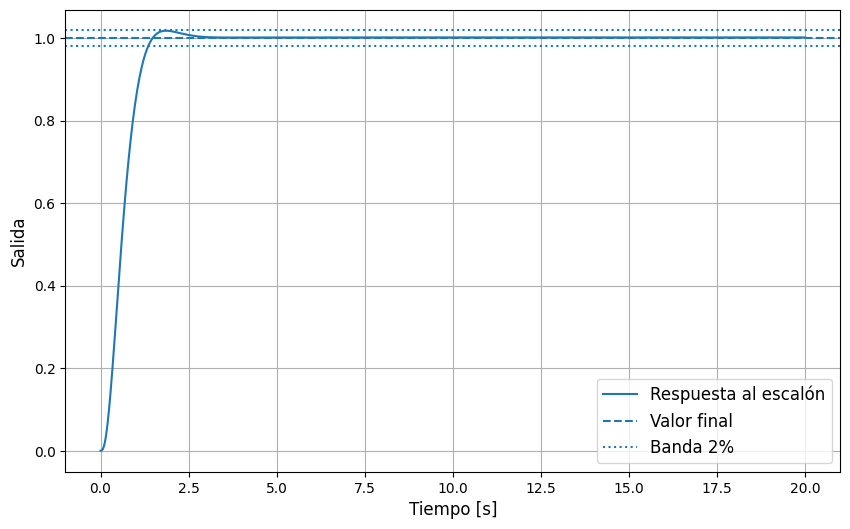
\includegraphics[width=0.90\textwidth]{figures/ej1_closed_loop_step_2.png}
  \caption{Respuesta al escalón unitario a lazo cerrado con compensador, con banda del $2\%$.}
  \label{fig:ej1_closed_loop_step_2}
\end{figure}

% -------------------------------------------------------
\subsubsection*{c) Márgenes del sistema compensado — Diagrama de Bode}
% -------------------------------------------------------

La Fig.~\ref{fig:ej1_bode} muestra el diagrama de Bode del sistema a lazo abierto con y sin el controlador PI.

\begin{figure}[H]
  \centering
  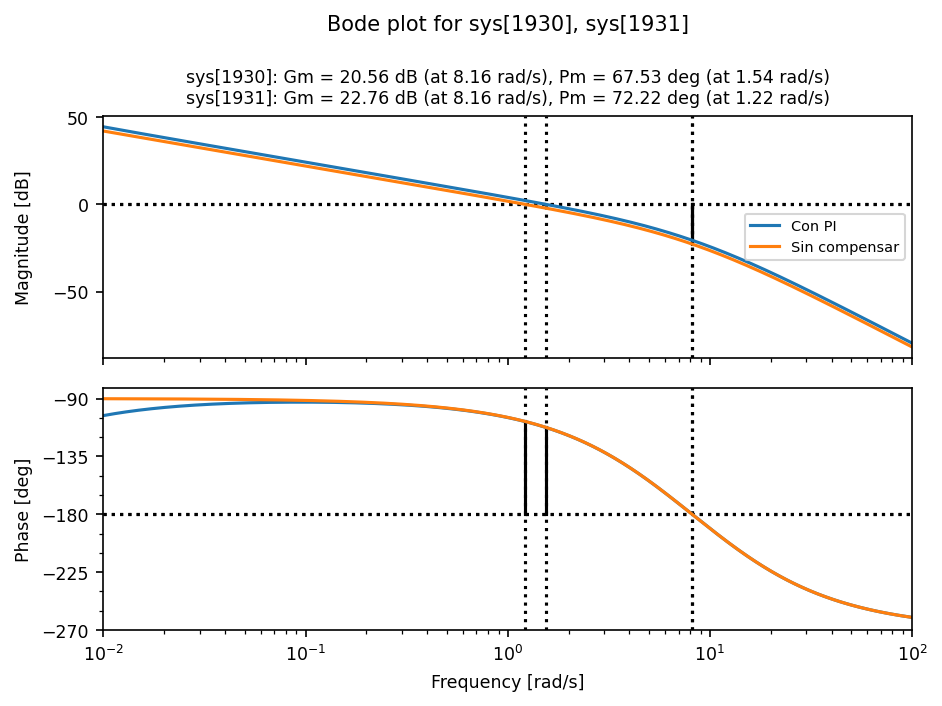
\includegraphics[width=0.90\textwidth]{figures/ej1_bode_comparison.png}
  \caption{Diagrama de Bode comparativo: sistema sin compensar vs.\ sistema con controlador PI.}
  \label{fig:ej1_bode}
\end{figure}

Al incorporar el controlador PI, ambos márgenes se reducen respecto al caso sin compensar (dado que el integrador añade $-90^\circ$ adicionales de fase en bajas frecuencias). Sin embargo, los márgenes resultantes son aún adecuados para garantizar estabilidad robusta.

% -------------------------------------------------------
\subsubsection*{d) Respuesta a la rampa unitaria con el controlador PI}
% -------------------------------------------------------

La Fig.~\ref{fig:ej1_ramp_pi} muestra la respuesta del sistema compensado ante una referencia rampa unitaria.

\begin{figure}[H]
  \centering
  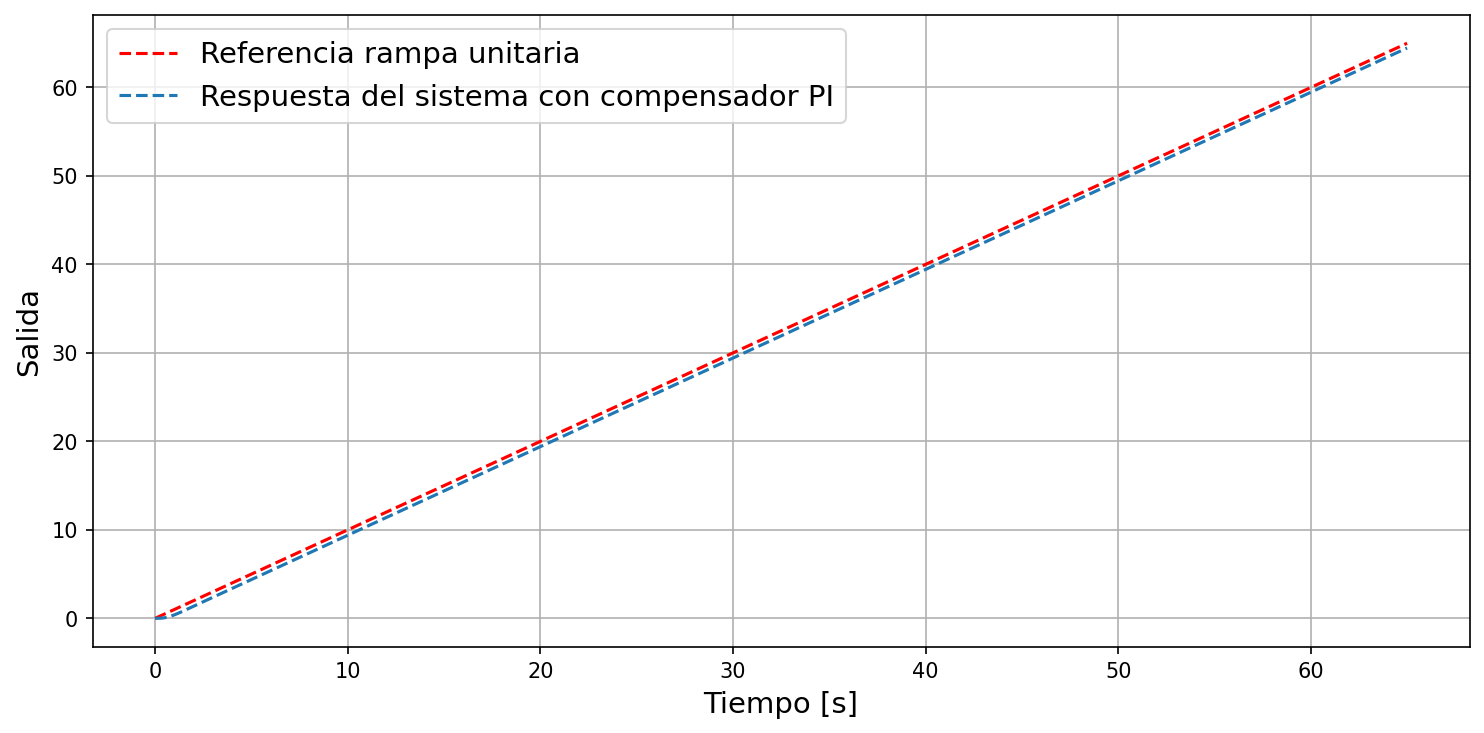
\includegraphics[width=0.85\textwidth]{figures/ej1_ramp_pi.png}
  \caption{Respuesta del sistema con controlador PI ante una referencia rampa unitaria.}
  \label{fig:ej1_ramp_pi}
\end{figure}

El error en estado estacionario ante la rampa es nulo, lo que se demuestra analíticamente:
Para una referencia rampa (\(R(s)=1/s^2\)) y una perturbación constante de magnitud $0.2$, definimos
\[
  E(s)=R(s)-\Theta(s)
\]
y
\[
  e_{ss}=\lim_{s\to 0} s\,E(s).
\]

Sustituyendo las expresiones de entrada y las funciones de transferencia:
\[
  e_{ss}=\lim_{s\to 0} s\left[\frac{1}{s^2} - \frac{\Theta(s)}{V(s)}\frac{1}{s^2} - \frac{\Theta(s)}{N(s)}\frac{0.2}{s}\right]
\]

Agrupando términos:
\[
  e_{ss}=\lim_{s\to 0}\left[\frac{s}{s^2}\left(1-\frac{\Theta(s)}{V(s)}\right) - \frac{\Theta(s)}{N(s)}\frac{0.2}{s}\right]
\]

Analizando el primer término del límite:
\[
  \lim_{s\to 0}\frac{1}{s}\left(1-\frac{\Theta(s)}{V(s)}\right)
\]

\[
  \lim_{s\to 0}\frac{1}{s}\left(1-\frac{\Theta(s)}{V(s)}\right)
  = \lim_{s\to 0}\frac{0.003s^3 + 0.0515s^2 + 0.2s}{0.003s^4 + 0.0515s^3 + 0.2s^2 + 0.25K_p s + 0.25K_i} =\frac{0}{0.25K_i}=0 \quad (K_i\neq 0).
\]

Ahora el término asociado a la perturbación:
\[
  \lim_{s\to 0}\frac{\Theta(s)}{N(s)}=\lim_{s\to 0}\frac{0.25s}{0.003s^4 + 0.0515s^3 + 0.2s^2 + 0.25K_p s + 0.25K_i}
  =\frac{0}{0.25K_i}=0 \quad (K_i\neq 0).
\]

Con esto, ambos contribuyentes al error en estado estacionario son nulos, por lo que
\[
  e_{ss}=0.
\]


% -------------------------------------------------------
\subsubsection*{e) Conclusión sobre el controlador}
% -------------------------------------------------------

Como se demuestra en el punto anterior, el controlador PI ya garantiza seguimiento con error nulo ante la referencia rampa, sin necesidad de modificaciones adicionales. Esto se debe a que el integrador del PI eleva el tipo del sistema de 1 a 2.

\newpage
% ====================================================================
\section{Ejercicio 2: Análisis y Control frente a Perturbaciones}
% ====================================================================

El sistema considerado en este ejercicio utiliza el modelo simplificado del actuador (sin dinámica eléctrica):
\[
  G(s) = \frac{\Theta(s)}{V(s)} = \frac{K}{s(Js+B)} = \frac{1}{s(s+B)}, \qquad K=1,\ J=1
\]

\subsection{Parte A: Análisis de Sensibilidad y Robustez}

% -------------------------------------------------------
\subsubsection*{a) Diagrama de Nyquist y estabilidad nominal ($B=0.5$)}
% -------------------------------------------------------

Para el sistema nominal con $B=0.5$, la función de transferencia es:
\[
  G(s) = \frac{1}{s^2+0.5s}
\]

El margen de fase nominal es $\text{MF} = 28.02^\circ$. La Fig.~\ref{fig:ej2_nyquist_nom} muestra el diagrama de Nyquist.

\begin{figure}[H]
  \centering
  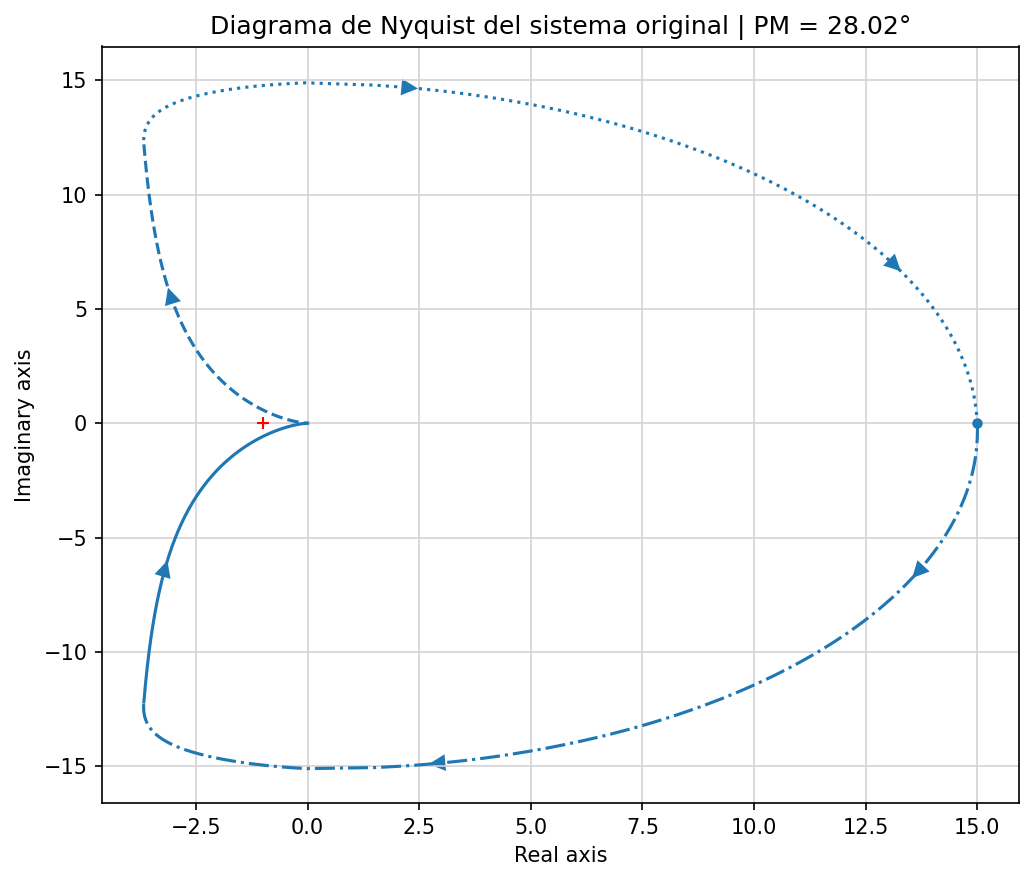
\includegraphics[width=0.65\textwidth]{figures/ej2_nyquist_nominal.png}
  \caption{Diagrama de Nyquist del sistema nominal ($B=0.5$) en lazo cerrado con realimentación unitaria.}
  \label{fig:ej2_nyquist_nom}
\end{figure}

Aplicando el criterio de estabilidad de Nyquist:
\begin{itemize}
  \item $P = 0$: la planta $G(s)$ no tiene polos en el semiplano derecho estricto (el polo doble en $s=0$ está sobre el eje imaginario y se rodea por un semicírculo de radio $\varepsilon\to 0$ que no encierra).
  \item $N = 0$: la curva de Nyquist no encierra al punto crítico $(-1, 0)$.
  \item $Z = N + P = 0$: el sistema en lazo cerrado no tiene polos en el semiplano derecho.
\end{itemize}

\textbf{Conclusión:} el sistema es \textbf{estable en lazo cerrado} para $B=0.5$.

% -------------------------------------------------------
\subsubsection*{b) Simulación con falla en $t=15\ \si{s}$}
% -------------------------------------------------------

Se simuló el sistema en lazo cerrado con referencia escalón unitario, considerando que en $t=15\ \si{s}$ el parámetro $B$ cambia de $0.5$ a $-0.1$. La Fig.~\ref{fig:ej2_fault} muestra el resultado.

\begin{figure}[H]
  \centering
  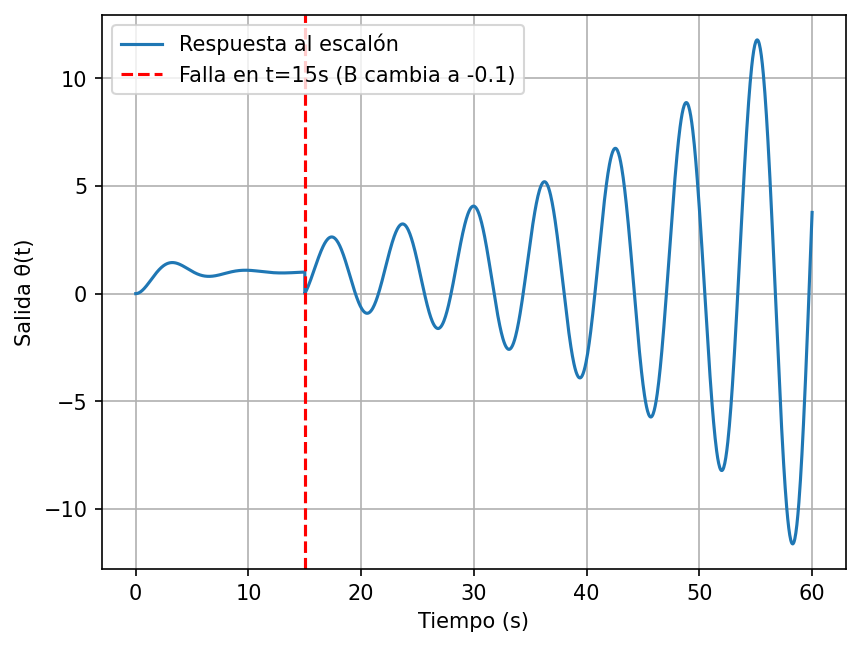
\includegraphics[width=0.75\textwidth]{figures/ej2_fault_response.png}
  \caption{Respuesta al escalón del sistema sin compensar: el parámetro $B$ cambia de $0.5$ a $-0.1$ en $t=15\ \si{s}$.}
  \label{fig:ej2_fault}
\end{figure}

Para $t < 15\ \si{s}$ el sistema opera correctamente y sigue la referencia. En el instante de la falla, la salida diverge exponencialmente: el sistema se vuelve \textbf{inestable}.

% -------------------------------------------------------
\subsubsection*{c) Root locus para $B=0.5$ y $B=-0.1$}
% -------------------------------------------------------

La Fig.~\ref{fig:ej2_rlocus} muestra el lugar de las raíces para ambos valores del parámetro $B$.

\begin{figure}[H]
  \centering
  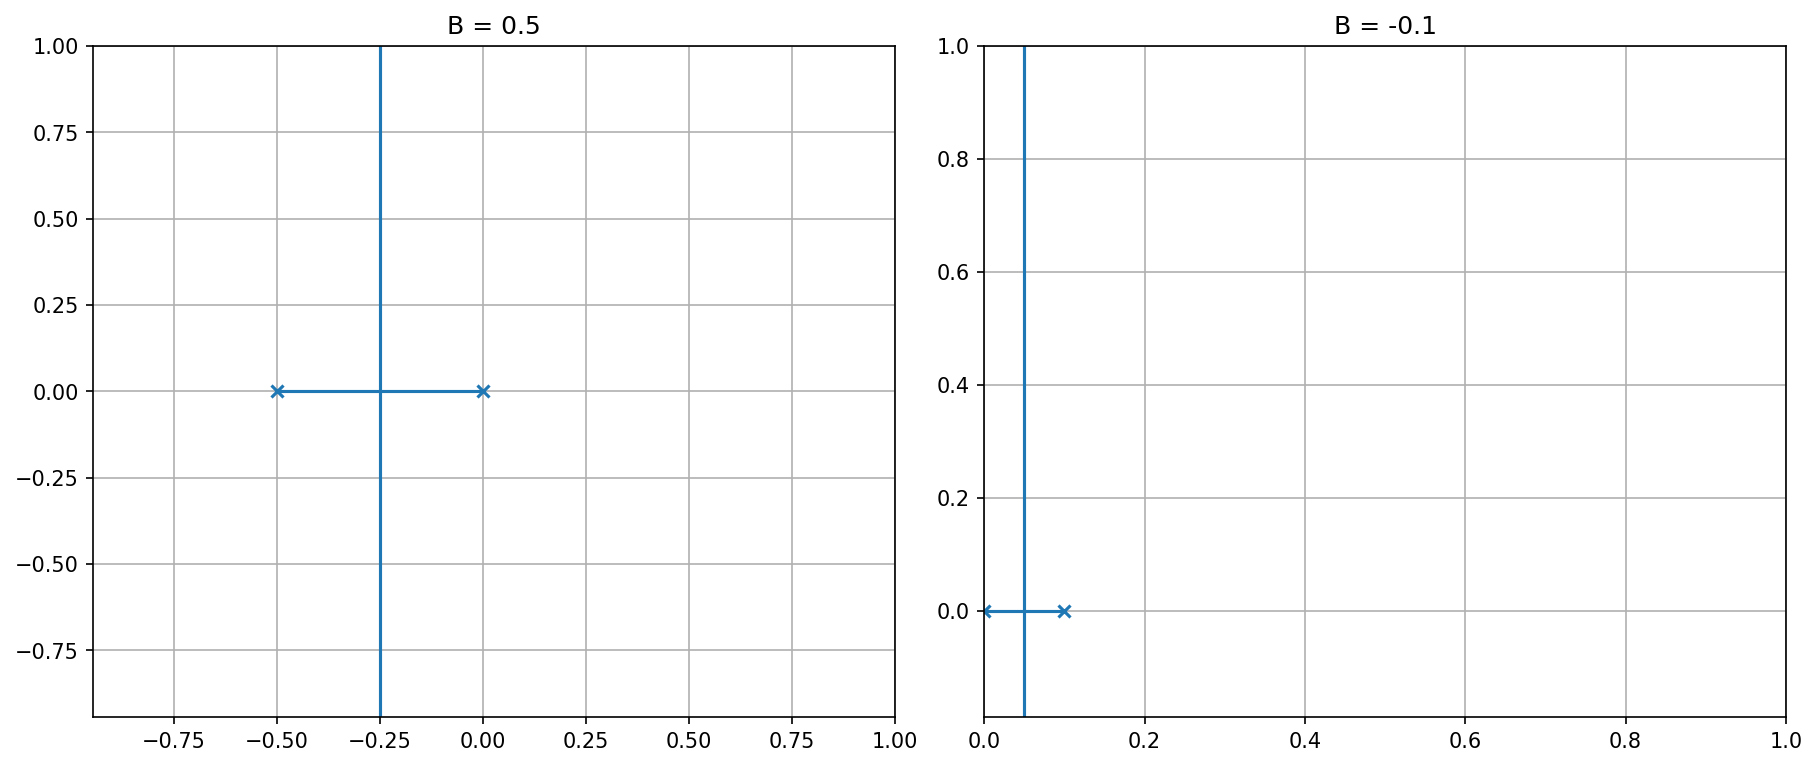
\includegraphics[width=0.90\textwidth]{figures/ej2_root_locus.png}
  \caption{Lugar de las raíces del sistema para $B=0.5$ (izquierda) y $B=-0.1$ (derecha).}
  \label{fig:ej2_rlocus}
\end{figure}

Con $B=0.5$, la planta a lazo abierto tiene polos en $s=0$ y $s=-B/J = -0.5$. Ambos polos están en el semiplano izquierdo (o en el eje imaginario), y el lugar de las raíces permanece en el semiplano izquierdo para valores positivos de ganancia, confirmando la estabilidad en lazo cerrado.

Con $B=-0.1$, el polo mecánico se desplaza a $s=+0.1$ (semiplano derecho). La planta ya tiene un polo inestable en lazo abierto ($P=1$), por lo que se requiere que el diagrama de Nyquist encierre al punto crítico exactamente una vez en sentido antihorario para estabilizar el lazo cerrado. Sin embargo, el sistema en lazo cerrado con realimentación unitaria simple no logra esa condición, resultando en $Z = 1$ y sistema inestable.

\textbf{Conclusión:} el sistema no tiene ninguna \emph{reserva de robustez} frente a variaciones negativas de $B$. Cualquier valor $B < 0$ traslada un polo al semiplano derecho, provocando inestabilidad en lazo cerrado. Es necesario un compensador que incremente el margen de fase del sistema nominal y cree un ``colchón'' de estabilidad suficiente para absorber esta degradación.

% -------------------------------------------------------
\subsubsection*{d) Tipo de compensador recomendado}
% -------------------------------------------------------

La Fig.~\ref{fig:ej2_bode_fault} compara los diagramas de Bode para $B=0.5$ y $B=-0.1$.

\begin{figure}[H]
  \centering
  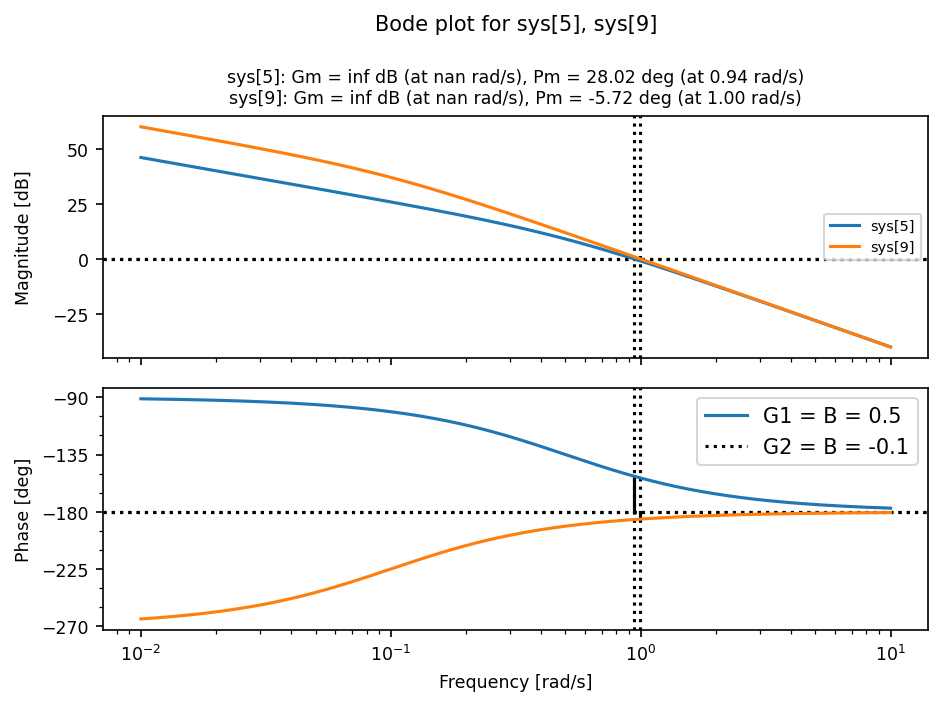
\includegraphics[width=0.85\textwidth]{figures/ej2_bode_fault.png}
  \caption{Diagrama de Bode comparativo: sistema nominal ($B=0.5$) vs.\ sistema con falla ($B=-0.1$).}
  \label{fig:ej2_bode_fault}
\end{figure}

Con $B=-0.1$ el margen de fase es \textbf{negativo}, confirmando la inestabilidad. Para otorgar al sistema un margen de seguridad ante la falla, se propone un \textbf{compensador lead (adelantador de fase)}.

El compensador \emph{lead} tiene la forma $C(s) = K_c\,\frac{s+z}{s+p}$ con $p > z > 0$, y su contribución es una \emph{fase positiva} en la región de cruce de ganancia. Esto incrementa directamente el margen de fase del sistema nominal, generando una reserva que permite tolerar la pérdida de fase producida por la degradación de $B$.

Un compensador \emph{lag} reduce la ganancia en altas frecuencias pero no agrega fase en el cruce, por lo que no resuelve el problema de margen. Un compensador \emph{lead-lag} también podría utilizarse, pero en este caso el objetivo es exclusivamente aumentar el margen de fase, por lo que el lead puro es suficiente y más simple de diseñar.

% ====================================================================
\subsection{Parte B: Diseño de Compensador para Estabilidad Robusta}
% ====================================================================

% -------------------------------------------------------
\subsubsection*{a) Diseño del compensador lead para MF = 35\ensuremath{^\circ}, 50\ensuremath{^\circ} y 65\ensuremath{^\circ}}
% -------------------------------------------------------

El compensador lead se parametriza como:
\[
  C(s) = K_c\,\frac{s + z}{s + p}, \qquad z = \alpha\,p,\quad 0 < \alpha < 1
\]

Para normalizar la ganancia en CC (y no alterar el error de posición del sistema), se impone $C(0) = 1$:
\[
  K_c = \frac{p}{z} = \frac{1}{\alpha}
\]

La fase máxima que puede aportar el compensador está relacionada con $\alpha$ mediante:
\[
  \alpha = \frac{1-\sin\phi_{\max}}{1+\sin\phi_{\max}}
\]

El margen de fase nominal del sistema es $\text{MF}_0 = 28.02^\circ$. Los incrementos de fase requeridos para cada objetivo son:

\begin{center}
\begin{tabular}{ccc}
  \toprule
  MF objetivo & Incremento requerido & $\phi_{\max,\text{diseño}}$ (con $+10^\circ$ de margen)\\
  \midrule
  $35^\circ$ & $6.98^\circ$  & $16.98^\circ$ \\
  $50^\circ$ & $21.98^\circ$ & $31.98^\circ$ \\
  $65^\circ$ & $36.98^\circ$ & $46.98^\circ$ \\
  \bottomrule
\end{tabular}
\end{center}

Para cubrir el caso más exigente ($\phi_{\max,\text{diseño}} \approx 47^\circ$) con un único valor de $\alpha$:
\[
  \alpha = \frac{1-\sin(47\ensuremath{^\circ})}{1+\sin(47\ensuremath{^\circ})} = 0.1552
\]

Dado $\alpha$, se realiza una búsqueda del polo $p$ que minimiza el error entre el margen de fase compensado y el objetivo. El gráfico de la Fig.~\ref{fig:ej2_lead_design} ilustra el proceso.

\begin{figure}[H]
  \centering
  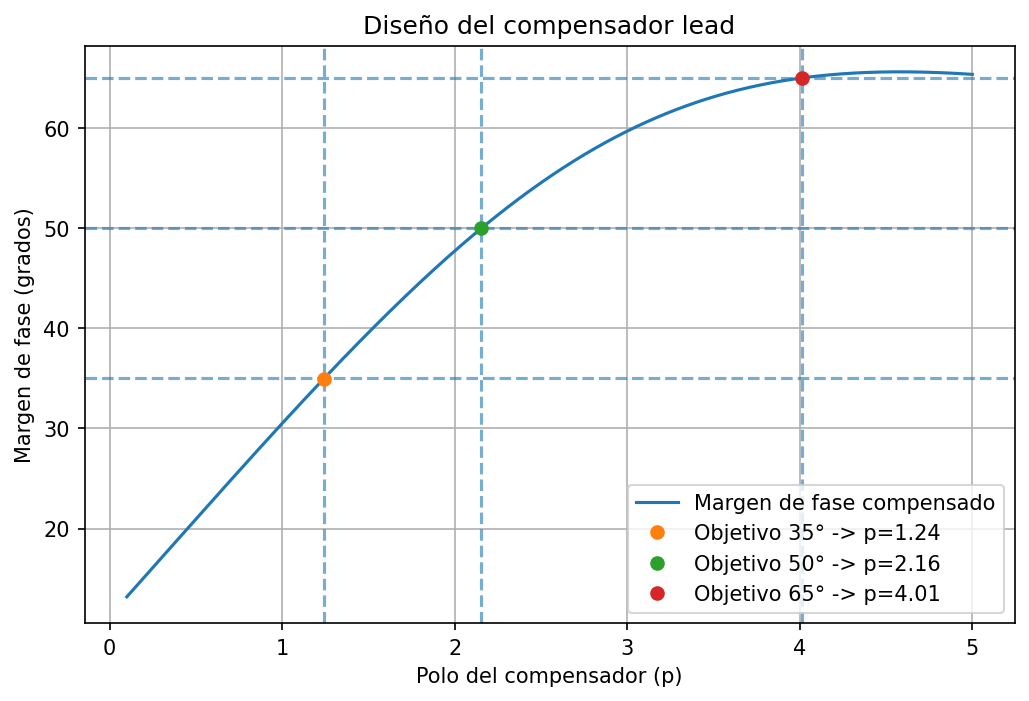
\includegraphics[width=0.75\textwidth]{figures/ej2_lead_design.png}
  \caption{Búsqueda del polo $p$ del compensador lead para cada objetivo de margen de fase.}
  \label{fig:ej2_lead_design}
\end{figure}

Los parámetros de los tres compensadores diseñados son:

\begin{center}
\begin{tabular}{cccc}
  \toprule
  MF objetivo & Polo $p$ & Cero $z = \alpha p$ & Ganancia $K_c = 1/\alpha$ \\
  \midrule
  $35^\circ$ & $1.24$ & $0.192$ & $6.44$ \\
  $50^\circ$ & $2.16$ & $0.335$ & $6.44$ \\
  $65^\circ$ & $4.01$ & $0.622$ & $6.44$ \\
  \bottomrule
\end{tabular}
\end{center}

% -------------------------------------------------------
\subsubsection*{b) Verificación mediante diagramas de Bode}
% -------------------------------------------------------

La Fig.~\ref{fig:ej2_bode_comp} presenta los diagramas de Bode del sistema compensado para los tres casos, confirmando los márgenes de fase obtenidos.

\begin{figure}[H]
  \centering
  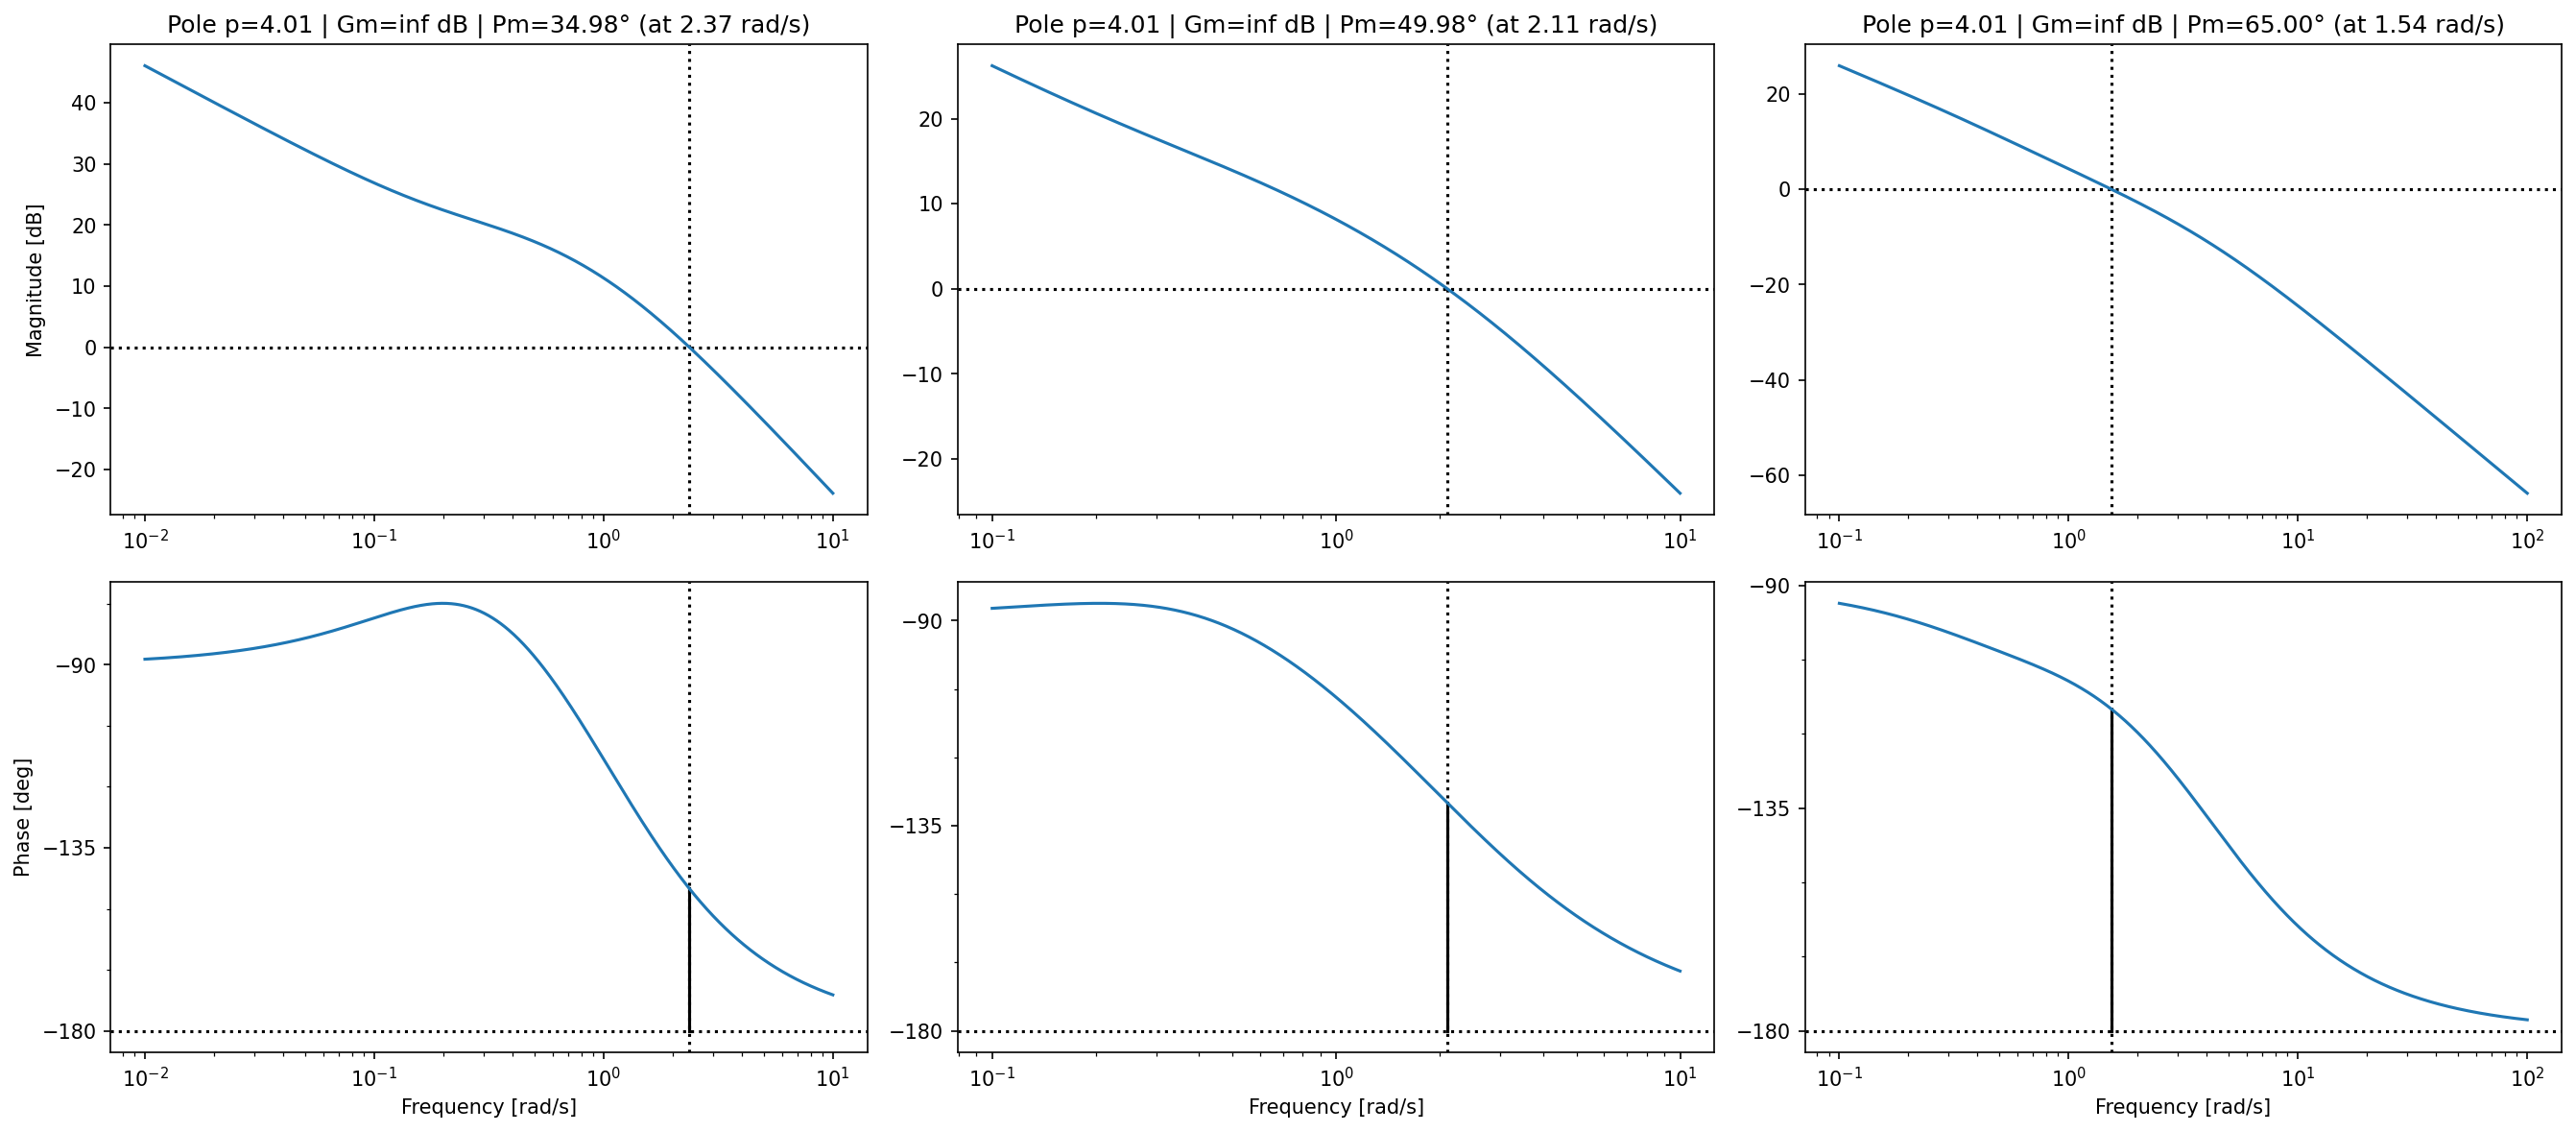
\includegraphics[width=\textwidth]{figures/ej2_bode_compensated.png}
  \caption{Diagramas de Bode del sistema nominal compensado para MF = 35\ensuremath{^\circ}, 50\ensuremath{^\circ} y 65\ensuremath{^\circ}. Se verifican los márgenes de fase requeridos y la normalización del compensador ($\text{ganancia DC} = 1$).}
  \label{fig:ej2_bode_comp}
\end{figure}

% -------------------------------------------------------
\subsubsection*{c) Respuesta al escalón con falla en $t=15\ \si{s}$}
% -------------------------------------------------------

La Fig.~\ref{fig:ej2_step_comp} muestra las respuestas al escalón para los tres compensadores, con la falla introducida en $t=15\ \si{s}$.

\begin{figure}[H]
  \centering
  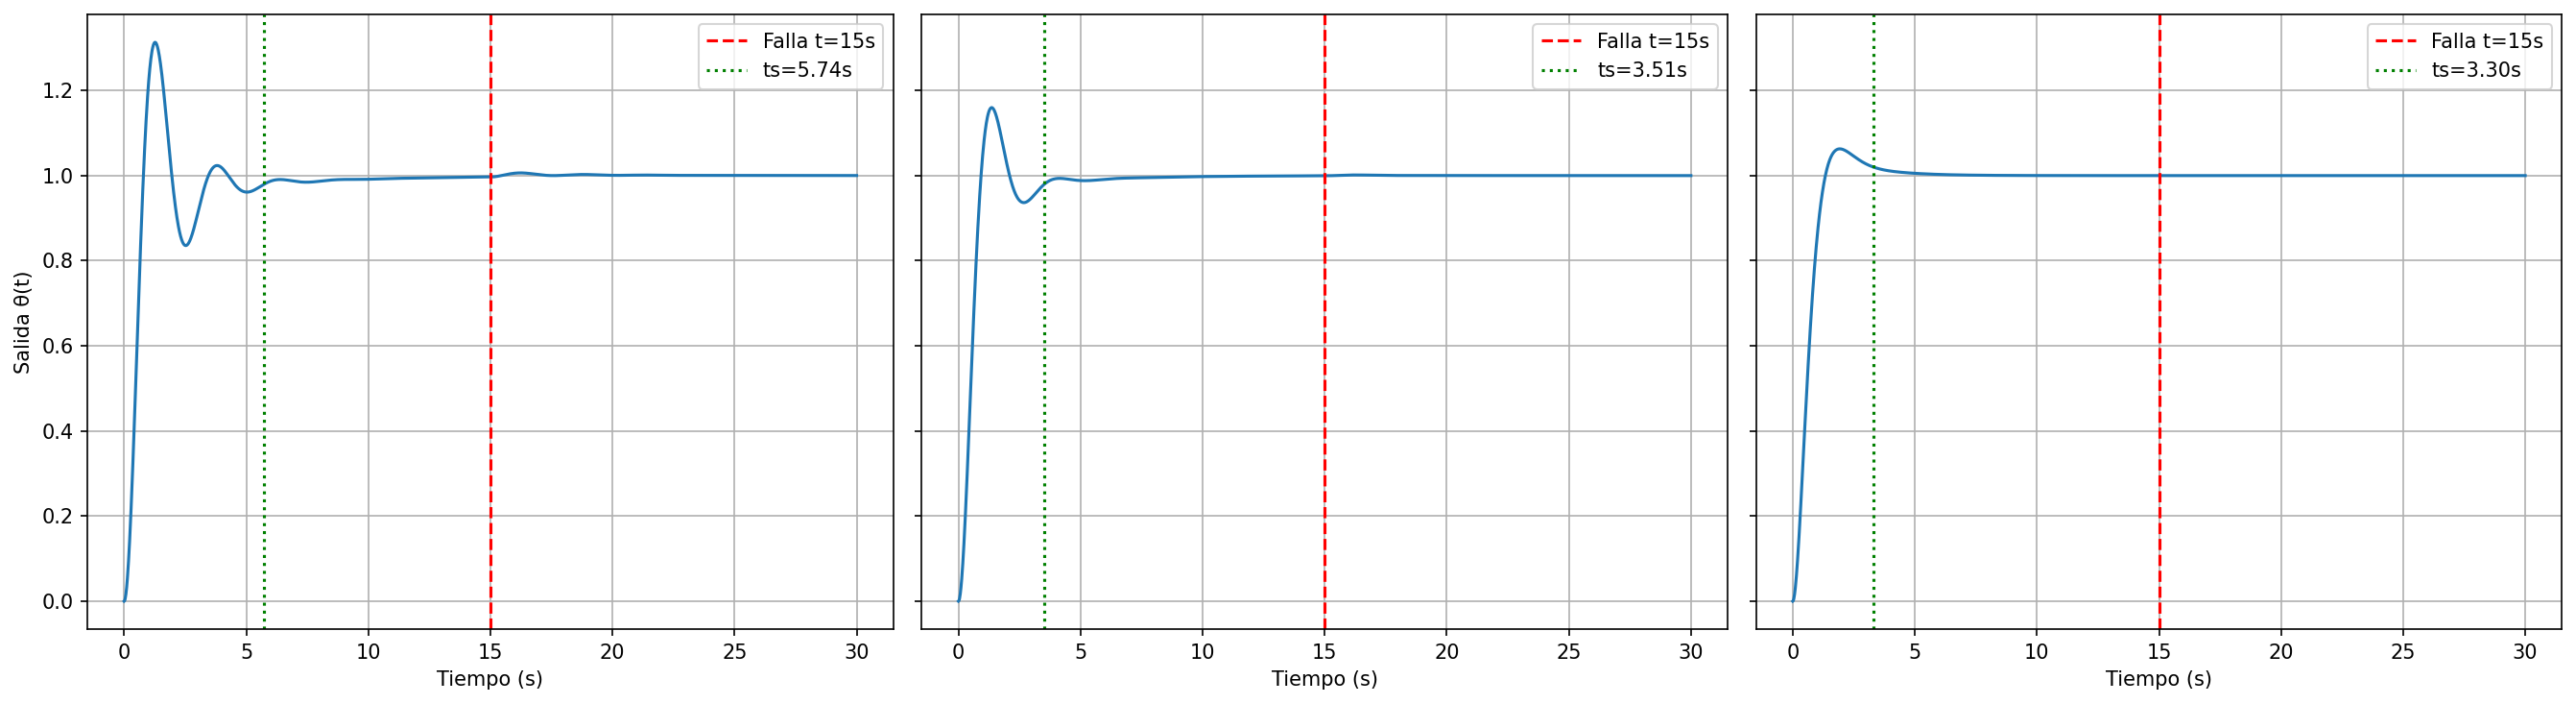
\includegraphics[width=\textwidth]{figures/ej2_step_fault_compensated.png}
  \caption{Respuesta al escalón del sistema compensado con falla en $t=15\ \si{s}$ ($B$ cambia de $0.5$ a $-0.1$). Los tres compensadores mantienen la estabilidad.}
  \label{fig:ej2_step_comp}
\end{figure}

A diferencia del caso sin compensar, en ninguno de los tres escenarios la falla produce divergencia. Los tiempos de establecimiento globales (medidos desde $t=0$) son:

\begin{center}
\begin{tabular}{ccc}
  \toprule
  Compensador & MF nominal & $t_s$ post-falla \\
  \midrule
  $p = 1.24$ & $35^\circ$ & $5.74\ \si{s}$ \\
  $p = 2.16$ & $50^\circ$ & $3.51\ \si{s}$ \\
  $p = 4.01$ & $65^\circ$ & $3.30\ \si{s}$ \\
  \bottomrule
\end{tabular}
\end{center}

Se observa que a mayor margen de fase, menor tiempo de establecimiento y menor sobreoscilación. Esto se debe a que un mayor MF implica un sistema más amortiguado. A medida que el MF aumenta hacia $65^\circ$, el sistema se asemeja progresivamente a un \textbf{sistema de primer orden}: la respuesta se vuelve monótona, sin rebotes perceptibles, con un transitorio suave tras la falla.

% -------------------------------------------------------
\subsubsection*{d) Diagrama de Nyquist del sistema compensado y desventajas}
% -------------------------------------------------------

\textbf{1) Análisis de Nyquist.}
La Fig.~\ref{fig:ej2_nyquist_comp} muestra los diagramas de Nyquist para los tres sistemas compensados.

\begin{figure}[H]
  \centering
  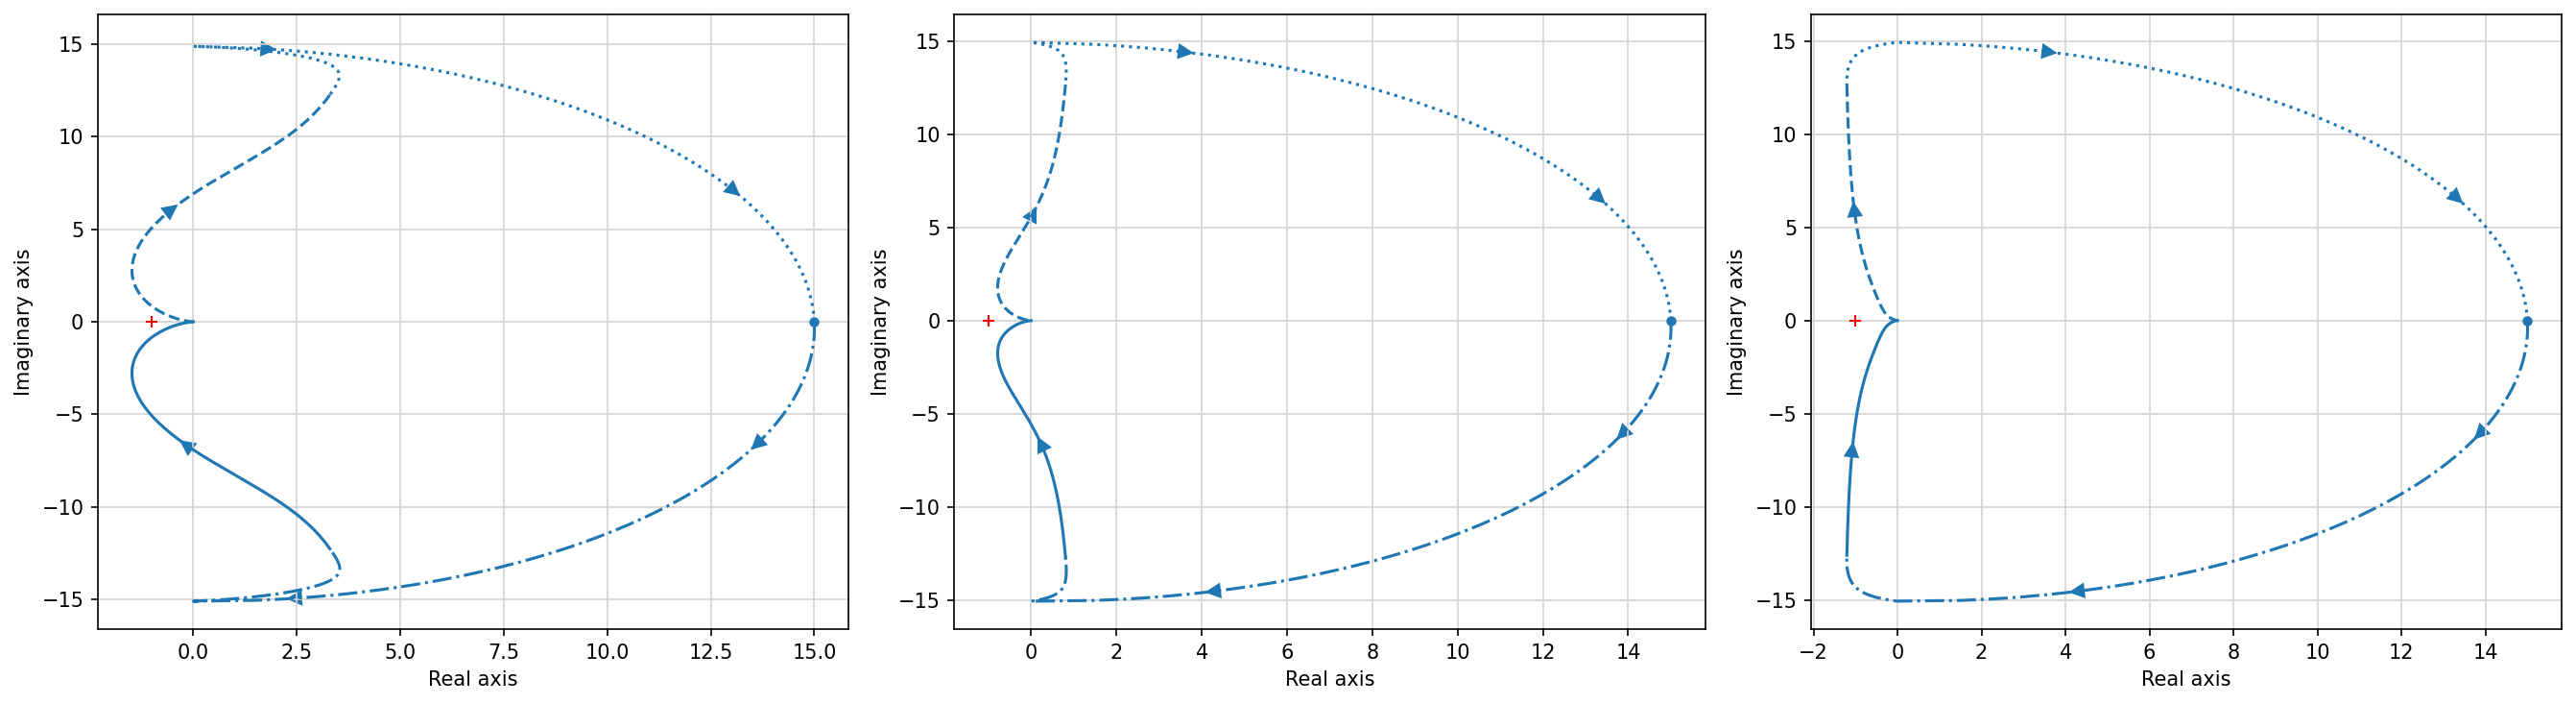
\includegraphics[width=\textwidth]{figures/ej2_nyquist_compensated.png}
  \caption{Diagramas de Nyquist del sistema compensado para los tres valores de MF.}
  \label{fig:ej2_nyquist_comp}
\end{figure}

En los tres casos la curva de Nyquist gira en sentido horario. El compensador lead produce una \emph{rotación de la curva} en la región de cruce de ganancia, alejándola del punto crítico $(-1, 0)$: cuanto mayor es el MF, mayor es la distancia mínima de la curva a dicho punto. Esta distancia adicional constituye la ``reserva de estabilidad'' que permite que la degradación física del parámetro $B$ —que equivale a un desplazamiento de la curva hacia el punto crítico— no cause inestabilidad.

\textbf{2) Desventajas de incrementar el MF.}
\begin{itemize}
  \item \textbf{Mayor polo $p$:} compensadores con MF más alto requieren polos más grandes, lo que amplifica el ruido de alta frecuencia y puede excitar dinámicas no modeladas.
  \item \textbf{Reducción del ancho de banda en lazo cerrado:} paradójicamente, el mayor amortiguamiento reduce el ancho de banda, lo que se traduce en una respuesta más lenta ante referencias:
  \begin{center}
  \begin{tabular}{cc}
    \toprule
    MF objetivo & Ancho de banda (rad/s) \\
    \midrule
    $35^\circ$ & $3.72$ \\
    $50^\circ$ & $3.37$ \\
    $65^\circ$ & $2.36$ \\
    \bottomrule
  \end{tabular}
  \end{center}
  \item \textbf{Diseño excesivamente conservador:} un MF muy elevado implica sobrea\-mor\-ti\-gua\-mien\-to en condiciones normales, sacrificando dinamismo sin que la falla llegue a ocurrir.
\end{itemize}

\end{document}
